\justifying
\chapter{Seminarios}
\section{Seminario 1. 19 de septiembre}
\begin{ejer}
    [1] Recuerda el atlas de $\mathbf S^ 2 \subset \mathbb R^3$ dado por las proyecciones ortogonales $\{U_i^{\pm}, \varphi_i^{\pm}\}_{i=1}^3$. Comprueba que la topolog\'ia inducida por la estructura diferenciable es la topolog\'ia
    inducida en $\bold S^2$ por la topolog\'ia usual de $\mathbb R^3$ .
    \begin{sol}
        Consideremos $\mathcal{T}_u = \{U \cap \bold{S}^2 \, / \, U \text{ abto de } \mathbb R^3 \}=$ topolog\'ia usual de $\mathbb R^3$ y $\mathcal{T}_e =$ topolog\'ia inducida por la estructura diferenciable. Una opci\'on es considerar la aplicaci\'on 
        $Id:(\bold{S}^2, \mathcal{T}_e) \longrightarrow (\bold{S}^2, \mathcal{T}_u)$ y demostrar que es homeomorfismo, es decir, continua, biyectiva, y con inversa continua. Otra opci\'on es ver que $\mathcal{T}_u \subseteq \mathcal{T}_e$ y que $\mathcal{T}_e\subseteq \mathcal{T}_u$. En clase vimos tambi\'en la propiedad de que $\mathcal{T}_e = \mathcal{T}_u \, \iff$ cada $\varphi_i^{\pm}: (U_i^{\pm}, \mathcal{T}_u) \longrightarrow \mathbb R^2$ es un homeomorfismo sobre su imagen entre abiertos. Tiraremos por aqu\'i.

        Analizamos el caso de $\varphi_3^{+}$. Sabemos que $\varphi_3^{+}( U_3^{+}) = \{(x,y) \in \mathbb R^3 \, / \, x^2 + y^2 < 1\}$ es abierto de $\mathbb R^2$ y $U_3^{+}$ es  claramente abierto de $\mathcal{T}_u$ por ser $\bold S^2 \cap \{z > 0\}$ y adem\'as $\varphi_3^{+}:  U_3^{+} \longrightarrow \varphi_3^{+}( U_3^{+})$. 

        Veamos que $\varphi_3^{+}: (U_3^{+}, \mathcal{T}_u) \longrightarrow \mathbb R^2$ es continua. Se tiene que $\varphi_3^{+} = \pi_{|_{U_3^+}}$ donde
        $$\begin{array}{rrcl}
             \pi : & \mathbb R^3 & \longrightarrow &  \mathbb R^2 \\
             & (x_1,x_2,x_3) & \longmapsto & (x_1,x_2)
        \end{array}$$
        que sabemos que es continua, y por tanto $\psi_3^+$ con $\mathcal{T}_u$ es continua. 

        Veamos ahora que $(\varphi_3^{+})^{-1}:  \varphi_3^{+}( U_3^{+})\longrightarrow  U_3^{+}$ es continua. Como $\varphi_3^{+}$ es biyectiva (sobre su inversa) esto es lo mismo que probar que $\varphi_3^{+}$ con $\mathcal{T}_u$ es abierta. 

        Como la topolog\'ia usual de $\mathbb R^3$ viene dada por la base $\{B(p,r)\}_{p \in \mathbb R^3, r>0}$ bastar\'a ver que $\forall p \in U_3^+$ y $\forall r>0$, $\varphi_3^{+}(B(p,r) \cap U_3^{+})$ es abierto. De esta forma, siendo $p=(x_o, y_o, z_o) \in U_3^+$
        $$B(p,r) \cap U_3^+ = \{(x,y,z) \in \mathbb R^3 \, / \, \sqrt{(x-x_o)^2 + (y-y_o)^2 + (z-z_o)^2} < r, \, x^2 + y^2 +z^2=1, \, z> 0\} =$$ $$=\{(x,y,z) \in \mathbb R^3 \, / \, \sqrt{(x-x_o)^2 + (y-y_o)^2 +  (\sqrt{1-x^2-y^2}-z_o)^2} < r, \, x^2 + y^2 +z^2=1, \, z> 0\} $$
        y entonces
        $$\varphi_3^{+}(B(p,r) \cap U_3^{+}) = \{(x,y) \, / \,\sqrt{(x-x_o)^2 + (y-y_o)^2 +  (\sqrt{1-x^2-y^2}-z_o)^2} < r, x^2 + y^2 < 1\}$$
        y como solo hay desigualdades estrictas, es un abierto de $\mathbb R^2$.  

    \end{sol}
\end{ejer}
\begin{ejer}
    [2] \textit{Parte del ejercicio 1.6}: Proyecci\'on estereogr\'afica. Considera la esfera
        $$\bold S^2 = \{(x_1,x_2,x_3) \, | \, x_1^2 + x_2^2 +x_3^2 = 1\} \subset \mathbb R^3$$
        Siendo $N = (0, 0, 1)$ el polo norte, define la aplicaci\'on $\varphi_N : \bold S^2 - \{N\} \to \mathbb R^2$ del   
        siguiente modo. Si $p \in \bold S^2 - \{N\}$, entonces $\varphi_N (p)$ es el punto de intersecci\'on de la
        recta que pasa por $N$ y $p$ con el plano de ecuaci\'on $x_3 = 0$ (identificando dicho plano con $\mathbb R^2$).
        \begin{enumerate}[a)]
            \item Calcula la expresi\'on an\'alitica de $\varphi_N$ y de su inversa.
            \begin{sol}
                Llamando $p=(x_1,x_2,x_3) \in \bold{S}^2$ el punto que deseamos proyectar, y $p'=(x,y,z=0)$ el proyectado, la recta que une $p, N$ y $p'$ tiene como vector director
                $$pN= (x_1,x_2,x_3) - (0,0,1)= (x_1, x_2, x_3-1)$$
                y por tanto, la ecuaci\'on de la recta ser\'a
                $$(0,0,1) + \alpha (x_1, x_2, x_3-1)$$
                y tenemos que encontrar $p'$, por lo que cortamos con el plano $(x,y,z=0)$:
                $$\begin{cases}
                    \alpha x_1 = x \\ \alpha x_2 = y \\ 1+\alpha(x_3-1) = 0 \Rightarrow \alpha = \dfrac{1}{1-x_3}
                \end{cases} 
                \Rightarrow \begin{cases}
                    x= \dfrac{x_1}{1-x_3} \\ y= \dfrac{x_2}{1-x_3} 
                \end{cases}$$
                de forma que ya tenemos defininda la aplicaci\'on como
                $$\begin{array}{rrcl}
                     \varphi_N : & \bold S^2 - \{N\} & \longrightarrow & \mathbb R^2  \\
                     &(x_1,x_2,x_3) & \longmapsto & (x,y)=\left( \dfrac{x_1}{1-x_3}, \dfrac{x_2}{1-x_3}\right) 
                \end{array}$$
                Dado ahora $p'=(x,y,0)$, la recta que lo une con $N$ es $(0,0,1) + \lambda (x,y,-1)$, y cortando con la esfera
                $$\begin{cases}
                    \lambda x = x_1 \\ \lambda y = x_2 \\ (1 - \lambda)^2 = x_3^2  \\ x_3 = \sqrt{1-x_1^2 - x_2^2} 
                \end{cases}$$
                y partiendo de la 3a ecuaci\'on
                $$ (1 - \lambda)^2  = 1-\lambda^2 x^2 -\lambda^2 y^2 \Rightarrow (1 - \lambda)^2  = 1-\lambda^2 (x^2 +y^2) \Rightarrow \lambda = \dfrac{2}{1 + x^2 + y^2}$$
                de forma que 
                $$\begin{cases}
                    x_1 = \dfrac{2x}{1 + x^2 + y^2} \\ x_2 = \dfrac{2y}{1 + x^2 + y^2} \\ x_3 =1-\dfrac{2}{1 + x^2 + y^2} = \dfrac{-1 + x^2 + y^2}{1 + x^2 + y^2}
                \end{cases}$$\
                teniendo as\'i definida la aplicaci\'on inversa:
                 $$\begin{array}{rrcl}
                     \varphi_N^{-1} : & \mathbb R^2 & \longrightarrow & \bold{S}^2  \\
                     &(x,y) & \longmapsto & (x_1,x_2,x_3) = \left( \dfrac{2x}{1 + x^2 + y^2} , \dfrac{2y}{1 + x^2 + y^2}, \dfrac{-1 + x^2 + y^2}{1 + x^2 + y^2}\right)
                \end{array}$$
            \end{sol}
            \item De un modo similar, define $\varphi_S: \bold S^2 - \{S\} \to \mathbb R^2$, donde $S=(0,0,-1)$ es el polo sur de la esfera.
            \begin{sol}
                Como lo \'unico que cambia es $S=(0,0,-1)$, las aplicaciones ahora son
                $$\begin{array}{rrcl}
                     \varphi_S : & \bold S^2 - \{S\} & \longrightarrow & \mathbb R^2  \\
                     &(x_1,x_2,x_3) & \longmapsto & (x,y)=\left( \dfrac{x_1}{x_3+1}, \dfrac{x_2}{x_3+1}\right) 
                \end{array}$$ 
                $$\begin{array}{rrcl}
                     \varphi_S^{-1} : & \mathbb R^2 & \longrightarrow & \bold S^2 - \{S\}  \\
                     & (x,y) & \longmapsto & (x_1,x_2,x_3) = \left( \dfrac{2x}{1 + x^2 + y^2} , \dfrac{2y}{1 + x^2 + y^2}, \dfrac{1 - x^2 - y^2}{1 + x^2 + y^2}\right)
                \end{array}$$
            \end{sol}
            \item Demuestra que las funciones de transici\'on son difeomorfismos.
            \begin{sol}
                Para ello, veamos que $\bold S^2 - \{N\} \cap \bold S^2 - \{S\} = \bold S^2 - \{N, S\}$ y comprobemos que $\varphi_N \circ \varphi_S^{-1}$ y $\varphi_S \circ \varphi_N^{-1}$ son difeomorfismos (diferenciable, biyectiva y con inversa diferenciable). En el primer caso, tenemos que se define la aplicaci\'on
                $$\begin{array}{rrrcll}
                     \varphi_N \circ \varphi_S^{-1} : & \mathbb R^2 = \varphi_N(\bold S^2 - \{N, S\}) & \overset{\varphi_S^{-1}}{\longrightarrow} & \bold S^2 - \{N, S\}& \overset{\varphi_N}{\longrightarrow} & \mathbb R^2 = \varphi_S(\bold S^2 - \{N, S\}) \\   
                \end{array}$$
                de forma que $$(x,y)  \longmapsto  \left( \frac{2x}{1 + x^2 + y^2} , \frac{2y}{1 + x^2 + y^2}, \frac{1 - x^2 - y^2}{1 + x^2 + y^2}\right) \longmapsto \left( \dfrac{x_1}{1-x_3}, \dfrac{x_2}{1-x_3}\right)$$
                y sustituyendo:
                $$\dfrac{x_1}{1-x_3}=\dfrac{\frac{2x}{1 + x^2 + y^2}}{1-\frac{1 - x^2 - y^2}{1 + x^2 + y^2}} = \dfrac{\frac{2x}{\cancel{1 + x^2 + y^2}}}{\frac{1+x^2+y^2-1 +x^2 + y^2}{\cancel{1 + x^2 + y^2}}} = \dfrac{2x}{2x^2 + 2y^2} =\dfrac{x}{x^2 + y^2}$$
                $$ \dfrac{x_2}{1-x_3} = \dfrac{y}{x^2 + y^2}$$
                    y entonces la expresi\'on en coordenadas de la funci\'on de transici\'on es
                    $$\begin{array}{rrcl}
                     \varphi_N \circ \varphi_S^{-1} : & \mathbb R^2 & \longrightarrow & \mathbb R^2 \\
                     & (x,y) & \longmapsto & \left(  \dfrac{x}{x^2 + y^2}, \dfrac{y}{x^2 + y^2}\right)
                \end{array}$$
                An\'alogamente, con $\varphi_S \circ \varphi_N^{-1}$ es, en coordenadas,
                $$(x,y) \overset{\varphi_N^{-1}}{\longmapsto} \left( \dfrac{2x}{1 + x^2 + y^2} , \dfrac{2y}{1 + x^2 + y^2}, \dfrac{-1 + x^2 + y^2}{1 + x^2 + y^2}\right)  \overset{\varphi_S}{\longmapsto} \left( \dfrac{x_1}{x_3+1}, \dfrac{x_2}{x_3+1}\right)  $$
                y sustituyendo en la \'ultima, 
                $$\dfrac{x_1}{x_3+1} = \dfrac{2x}{1 + x^2 + y^2 - 1 + x^2 + y^2} = \dfrac{x}{x^2+y^2}$$
                $$\dfrac{x_2}{x_3+1} = \dfrac{y}{x^2 + y^2}$$
                teniendo la misma expresi\'on que la funci\'on de transici\'on anterior. Adem\'as,  $\varphi_N \circ \varphi_S^{-1}$ tiene como inversa $(\varphi_N \circ \varphi_S^{-1})^{-1} = \varphi_S \circ \varphi_N^{-1}$, es decir, una es inversa de la otra y viceversa. Basta entonces comprobar que una es diferenciable, ya que ser\'a biyectiva por tener inversa. En efecto, son diferenciables, ya que lo son componente a componente, el denominador nunca es $0$ ya que $x^2+y^2 = 0 \iff x=0 \wedge y=0$ y no existe punto de la esfera que al unirlo con un polo su recta pase por $(0,0,0)$, ser\'ian los polos, pero los hemos eliminado por no estar definida la funci\'on de transici\'on en ellos.
            \end{sol}
            \item Concluye que $\{(\bold S^2 -\{N\}, \varphi_N), (\bold S^2 -\{S\}, \varphi_S)\}$ determina una estructura diferenciable sobre $\bold S^2$. 
            \begin{sol}
               Las parejas $\{(\bold S^2 -\{N\}, \varphi_N), (\bold S^2 -\{S\}, \varphi_S)\}$ son cartas, pues $\varphi_{N,S}$ son epiyectivas y $\varphi_{N,S}(\bold S^2 -\{N,S\}) = \mathbb R^2 - \{0\}$ es abierto. Para que sea un atlas, basta ver que los dominios recubren (en efecto, $\bold S^2 = \bold S^2 -\{N\} \cup \bold S^2 -\{S\}$) y las cartas son compatibles ($\varphi_{N,S}(\bold S^2 -\{N,S\})$ son abiertos como sea ha visto en la condici\'on de carta y se ha comprobado la diferenciablidad de las funciones de transici\'on en el apartado anterior). As\'i,concluimos que este atlas ``pequeño'' generará una estructura diferenciable, un atlas más grande compatible con todas las cartas de esa estructura. A continuación, comprobaremos que es el mismo que genera el atlas de las proyecciones ortogonales.
            \end{sol}
            \item Demuestra que esta estructura diferenciable es la misma que la que genera el atlas de las proyecciones ortogonales.
            \begin{sol}
                Dos atlas que generan el mismo atlas maximal son lo que llamamos equivalentes. Esto quiere decir que toda carta de un atlas es compatible con todas las cartas del otro. Haremos un caso, el dado por $(\bold S^2 -\{N\}, \varphi_N)$ y $(U_3^+, \psi_3^+)$. Dado que $\bold S^2 -\{N\}\cap U_3^+ =U_3^+ -\{N\} \neq \emptyset$, la compatibilidad viene dada al comprobar:
                \begin{enumerate}[1)]
                    \item $\varphi_N (U_3^+ -\{N\})$ y $\psi_3^+(U_3^+ -\{N\})$ son abiertos. El primer caso es el conjunto:
                    $$\varphi_N (U_3^+ -\{N\}) = \{(x,y) \, / \, x^2 + y^2 > 1\}$$
                    y la desigualdad es estricta por ser $U_3^+$ abierto, de forma que es abierto. En el segundo caso, 
                    $$\psi_3^+ (U_3^+ -\{N\}) = \{(x,y) \, / \, x^2 + y^2 < 1, x > 0, y > 0\}$$
                    que tambi\'en es abierto por ser todas las desigualdades estrictas.
                    \item Las funciones de transici\'on son diferenciables. Ahora estas funciones son $\varphi_N \circ \psi_3^{+^{-1}}$ y $\psi_3^+ \circ \varphi_N^{-1}$. Tenemos sus expresiones anal\'iticas, luego podemos hallar la expresi\'on de las composiciones
                    $$\varphi_N \circ \psi_3^{+^{-1}} (x,y) = \varphi_N (\psi_3^{+^{-1}} (x,y)) = \varphi_N (x,y,\sqrt{1-x^2 - y^2}) = $$
                    $$=\left( \dfrac{x}{1-\sqrt{1-x^2 - y^2}}, \dfrac{y}{1-\sqrt{1-x^2 - y^2}} \right) $$
                    y de la misma forma, 
                    $$\psi_3^+ \circ \varphi_N^{-1}(x,y)=\psi_3^+(\varphi_N^{-1}(x,y))=\psi_3^+\left(\dfrac{2x}{1 + x^2 + y^2} , \dfrac{2y}{1 + x^2 + y^2}, \dfrac{-1 + x^2 + y^2}{1 + x^2 + y^2}\right) =$$ $$= \left(\dfrac{2x}{1 + x^2 + y^2} , \dfrac{2y}{1 + x^2 + y^2} \right)$$
                    que por ser ambas (componente a componente) composci\'on, suma, resta y cociente de aplicaciones diferenciables, lo son, excepto quiz\'a donde se anule el denominador. Estudiemos ambos casos.

                    $$1-\sqrt{1-x^2 - y^2} = 0 \iff x^2 + y^2 = 0 \iff x = 0 \wedge y = 0$$
                    lo cual no es posible porque el punto $(0,0)$ hemos visto que es la imagen de los polos.
                    $$1 + x^2 + y^2 = 0 \iff x^2 + y^2 = -1$$
                    Tampoco es posible ya que no tiene soluciones reales.
                \end{enumerate}
            \end{sol}
        \end{enumerate}
\end{ejer}
\section{Seminario 2. 26 de septiembre}
\begin{ejer}
    [1] \textit{La banda de Moebius}. En $[0, 1] \times (0, 1) \subset \mathbb R^2$ considera la relaci\'on de equivalencia dada por: $$(x, y) \sim (z, t) \iff (x, y) = (z, t) \quad \text{\'o} \quad \begin{cases}
        x=0 \\ z=1 \\ y=1-t
    \end{cases} \quad \text{\'o}\quad  \begin{cases}
        x=1 \\ z=0 \\ y=1-t
    \end{cases}
    $$
Es decir, identificamos los lados derecho e izquierdo del cuadrado unidad, con distintas orientaciones:
$$\begin{tikzpicture}[scale=1.5, domain=-2:2, samples=70]
	
	% draw function
    \draw[black, thick] (-1,-1) -- (-1,1);
    \draw[->, black] (-1,-1) -- (-1,0);
    \draw[dashed, black] (-1,1) -- (1,1);
    \draw[black, thick] (1,1) -- (1,-1);
    \draw[->, black] (1,1) -- (1,0);
    \draw[dashed, black] (1,-1) -- (-1,-1);
    \end{tikzpicture} \qquad \qquad
    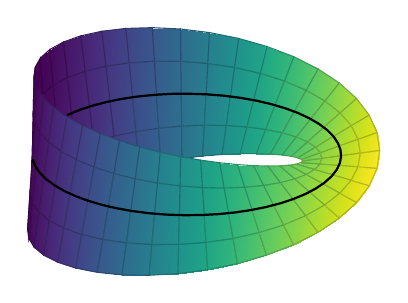
\begin{tikzpicture}
\begin{axis}[scale=0.75,
    hide axis,
    view={10}{40}
]
\addplot3 [
    surf, shader=faceted interp,
    point meta=x,
    colormap/viridis,
    samples=40,
    samples y=5,
    z buffer=sort,
    domain=0:360,
    y domain=-0.5:0.5
] (
    {(1+0.5*y*cos(x/2)))*cos(x)},
    {(1+0.5*y*cos(x/2)))*sin(x)},
    {0.5*y*sin(x/2)});

\addplot3 [
    samples=50,
    domain=-165:150, % The domain needs to be adjusted manually, depending on the camera angle, unfortunately
    samples y=0,
    thick
] (
    {cos(x)},
    {sin(x)},
    {0});
\end{axis}
\end{tikzpicture}$$

    Sea $M = \modulo{([0, 1] \times (0, 1))}{\sim}$ el conjunto de las clases de equivalencia. Considera los subconjuntos $U = \modulo{((0, 1) \times (0, 1))}{\sim}$ y $V =  \modulo{([0, 1] - \{\nicefrac{1}{2}\} \times (0, 1))}{\sim}$. Sean las aplicaciones $\varphi : U \to \mathbb R^2$ y $\psi : V \to \mathbb R^2$ dadas por: 
    $$\varphi([(x,y)]) = (x,y) \qquad \text{ y } \qquad \psi([(x,y)])=\begin{cases}
        (x,y) & \text{ si } x < \nicefrac{1}{2} \\  (x-1,1-y) & \text{ si } x > \nicefrac{1}{2} 
    \end{cases}.$$
    \begin{enumerate}
        \item Demuestra que $\{(U, \varphi), (V, \psi)\}$ es un atlas de $M$.
        \begin{sol}
            En primer lugar, comprobaremos que son cartas. Las aplicaciones ets\'an bien definidas, son inyectivas y las im\'agenes de los subconjuntos son abiertos. En efecto, $\varphi$ est\'a bien definida, pues $(x,y)\sim (x,y)$ solo, por habernos deshecho de los extremos. Adem\'as es inyectiva, ya que $\varphi([(x,y)]) = \varphi \circ \pi (x,y) =(x,y)$, es decir, $\varphi \circ \pi = Id$. As\'i pues, sobre $[0, 1] \times (0, 1)$, se verifica que $\varphi = \pi^{-1}$, luego por ser $\pi$ epiyectiva, $\varphi$ es inyectiva.
            
             $\psi$ est\'a bien definida. Si $x \neq 0,1$ las clases solo tienen un representante. Si $[(0,y)]=[(1,1-y)]$, entonces por $\psi$, $(0,y) = (0,1-(1-y))=(0,y)$
             
            De la misma forma pque en $\varphi$, se demuestra la inyectividad para $\psi$ si $x < \nicefrac{1}{2}$. En el caso en que $x > \nicefrac{1}{2}$, podemos argumentar, en el sentido m\'as elemental de inyectividad que
            $$\psi([(x,y)]) = \psi([(x',y')]) \iff (x-1,1-y)=(x'-1,1-y') \iff  $$
            $$\begin{cases}
                x-1=x'-1 & \Rightarrow x=x' \\ 1-y = 1-y' & \Rightarrow y=y'
            \end{cases} \implies (x,y) \sim (x',y') \iff [(x,y)] = [(x',y')]$$
            Adem\'as, 
            $$\varphi(U)=\pi^{-1}(U) =(0,1) \times (0,1) \qquad \psi(V)= (-\nicefrac{1}{2},\nicefrac{1}{2})  \times (0,1)$$
            que son abiertos en la topología producto (abierto $\times$ abierto).

            El segundo caso se demuestra como sigue:
            \begin{enumerate}
                \item En el conjunto $V_1=\modulo{[0,\nicefrac{1}{2}) \times (0,1)}{\sim}$, es el mismo caso que el anterior, luego 
                $$\psi(V_1) = [0,\nicefrac{1}{2}) \times (0,1)$$
                \item En el conjunto $V_2=\modulo{(\nicefrac{1}{2},1] \times (0,1)}{\sim}$, la aplicaci\'on es $\psi\circ \pi(x,y) = (x-1,1-y)$ de forma que 
                $$\psi(V_2)=(\nicefrac{1}{2}-1,1-1] \times (1,0) = (-\nicefrac{1}{2},0] \times (0,1)$$
            \end{enumerate} 
            de manera que
            $$\psi(V) = \psi(V_1 \cup V_2) = \psi(V_1) \cup \psi(V_2) = [0,\nicefrac{1}{2}) \times (0,1) \cup (-\nicefrac{1}{2},1] \times (0,1) =(-\nicefrac{1}{2},\nicefrac{1}{2}) \times (0,1)$$

            Comprobemos que son atlas. Claramente, $M = U \cup V$ ya que uno cubre lo que otro no. Para comprobar la compatibilidad de la funciones veamos sus inversas. 
            $$\bt 
            \varphi^{-1} : & (0,1) \times (0,1) \arrow{r} & U \\[-5mm] & (x,y) \arrow[mapsto]{r} & \left[(x,y)\right] \\ \psi^{-1}: & (-\nicefrac{1}{2},\nicefrac{1}{2}) \times (0,1) \arrow{r} & V \\[-8mm] 
            & (x,y) \arrow[mapsto]{r} & \begin{cases}
                [x,y] \quad \quad \quad 0 \leq x < \nicefrac{1}{2} \\ [x+1, 1-y] \quad -\nicefrac{1}{2} < x \leq 0
            \end{cases}
            \et$$
            y ahora $U \cap V = \modulo{((0, 1) - \{\nicefrac{1}{2}\} \times (0, 1))}{\sim}$, de forma que 
            $$\psi \circ \varphi^{-1}(x,y) = \psi([x,y])=\begin{cases}
                (x,y) & 0< x< \nicefrac{1}{2} \\ (x-1,1-y)& \nicefrac{1}{2}< x < 1
            \end{cases}$$
            que es diferenciable $\mathcal C^{\infty}$, ya que lo es cada componente conexa, excluyendo $0,1, \nicefrac{1}{2}$. De la misma forma
            $$\varphi^{-1} \circ \psi (x,y)=\begin{cases}
                (x,y) & 0< x< \nicefrac{1}{2} \\ (x-1,1-y)& -\nicefrac{1}{2}< x < 0
            \end{cases}$$
            es tambi\'en diferenciable, y $\{(U,\varphi),(V,\psi)\}$ es un atlas 2-dimensional $\mathcal{C}^{\infty}$ de $M$, pudiendo extenderlo a uno mayor maximal respecto a la condici\'on de compatibilidad.
        \end{sol}
        \item Analiza si est\'an bien definidas y son diferenciables las aplicaciones $f_i : M \to \mathbb R$, $i = 1, 2, 3$, dadas por:
        $$f_1([(x,y)])=y \quad f_2([(x,y)]) = (y-\nicefrac{1}{2})^2 \quad f_3([(x,y)])=\sin(\pi x) \cos(\pi y)$$
        \begin{sol}
            \begin{enumerate}
                \item No est\'a bien definida, ya que para $[(0,\nicefrac{1}{3})] = [(1,\nicefrac{2}{3})]$, $f_1$ asocia a ellos distintas im\'agenes.
                \item Sea una clase con dos respresentantes, $[(0,y)] = [(1,1-y)]$, de forma que su imagen es 
                $$(y-\nicefrac{1}{2})^2 =(1-y-\nicefrac{1}{2})^2 = (\nicefrac{1}{2}-y)^2$$ por lo que est\'a bien definida.
                Veamos si son diferenciables:
                $$f_2 \circ \varphi^{-1}(x,y)=f_2[x,y]=(y-\nicefrac{1}{2})^2$$
                $$f_2 \circ \psi^{-1}(x,y)=\begin{cases}
                    f_2[x+1,1-y] \\ f_2[x,y]
                \end{cases} = \begin{cases}
                    (1-y-\nicefrac{1}{2})^2 & 0\leq x< \nicefrac{1}{2} \\ (y-\nicefrac{1}{2})^2 &  -\nicefrac{1}{2}< x \leq0 
                \end{cases}= (y-\nicefrac{1}{2})^2$$
                que como hemos visto en el caso anterior, es diferenciable. 
                
                \textit{Observaci\'on.} Podr\'ia parecer que no es diferenciable por no coincidir los valores en el punto en el que no est\'a definido, pero es que este abierto total no es conexo, por lo que basta que sea diferenciable en cada componente conexa.
                \item Debería ser diferenciable.
            \end{enumerate}
        \end{sol}
        \item Determina si $g: M \to M$ est\'a bien definida y es diferenciable, donde:
        $$g([(x,y)]) = \left[\left(x,\nicefrac{1}{2}\right)\right]$$
        \begin{sol}
            Tenemos dos casos para $[(x,y)]$. Si $x \neq 0, 1$, entonces est\'a trivialmente bien definida, pues si $(x,y) \sim (x',y')$, entonces $(x,y) =(x',y')$. Ahora bien, si $x=0$, entonces $[x,y] = [x',y']$ con $x'=1$ e $y'=1-y$, es decir, $[(0,y)]=[(1,1-y)]$. Hagamos pues ambas im\'agenes por $g$ es decir, $g[(0,y)]=[(0,\nicefrac{1}{2})]$ y $g[(1,1-y)]=[(1, \nicefrac{1}{2})]$. Adem\'as, est\'an relacionados, ya que $\nicefrac{1}{2} = 1-\nicefrac{1}{2}$. Tambi\'en $g([x,y]) \in M$. As\'i concluimos que est\'a bien definida. 

            Para demostrar la diferenciabilidad, hacemos la composici\'on con la inversa de las cartas, si $p=[x,y] \in U$, entoces $g(p)\in U $podemos utilizar la lectura en coordenadas, es decir
            $$\varphi \circ g \circ \varphi^{-1}(x,y) = \varphi\circ g([x,y]) = \varphi([(x,\nicefrac{1}{2})])=(x,\nicefrac{1}{2})$$
            Para los $p=[0,y] \in V$, $g(p) \in V$
            $$\psi \circ g \circ \psi^{-1}(x,y) = \begin{cases}
                \psi (g([(x+1,1-y)]))  \\ 
                \psi (g([(x,y)]))     
            \end{cases} = \begin{cases}
                \psi([(x+1,\nicefrac{1}{2})])  &  \text{ si }-\nicefrac{1}{2}< x \leq 0   \\ 
                \psi([(x,\nicefrac{1}{2})])     & \text{ si }0\leq x< \nicefrac{1}{2} 
            \end{cases} $$
            $$=(x,\nicefrac{1}{2})$$
            que son diferenciables.
        \end{sol}
    \end{enumerate}
\end{ejer}
\section{Seminario 3. 3 de octubre}
\begin{ejer} [2]
    \textit{Ejercicio 1.18.} En el espacio vectorial de las matrices cuadradas $Mat_{n\times n}(\mathbb R)$ demuestra que son diferenciables las aplicaciones: suma de matrices, producto de
    matrices, trasposici\'on, traza y determinante. Demuestra que $GL(n, \mathbb R) = \{A \in Mat_{n\times n}(\mathbb R) \, / \, det A \neq 0 \}$ es un abierto de $Mat_{n\times n}(\mathbb R)$.
\end{ejer}
\begin{sol}
    Dado que $Mat_{n \times n}(\mathbb R) \simeq \mathbb R^{n^2}$, dotaremos a $Mat_{n \times n}(\mathbb R)$ de la estructura diferenciable generada por el atlas usual de $\mathbb R^{n^2}$, que es $\{(\mathbb R^{n^2}, Id)\}$. As\'i pues, para comprobar que son diferenciables las aplicaciones no hace falta ni comprobar la composici\'on, pues la \'unica carta del atlas es $(\mathbb R^{n^2}, Id)$. 

    Tambi\'en podemos definir la base est\'andar $\{E_{ij}\}_{1\leq i,j \leq n}$ siendo $E_{ij}$ la matriz con todo ceros y un 1 en el lugar $ij$ y para $A=(a_{ij})$ la aplicaci\'on $\varphi(A)=(a_{11}, \ldots, a_{nn})$ (el isomorfismo.)
    
    Usando el isomorfismo mencionado, podremos expresar las aplicaciones en coordenadas, por la correspondencia:
    $$Mat_{n \times n}(\mathbb R)  \ni\begin{pmatrix} a_{11} & \cdots & a_{1n} \\ \vdots & \ddots & \vdots \\ a_{n1} & \cdots & a_{nn} 
    \end{pmatrix} \leadsto (a_{11}, \ldots, a_{1n}, a_{21},  \ldots,  a_{2n}, \ldots, a_{n1}, \ldots, a_{nn} ) \in \mathbb R^{n^2}$$
    as\'i, tenemos las siguientes aplicaciones:
    \begin{itemize}
        \item Suma de matrices
        $$f(A,B) = A+B = (a_{ij} + b_{ij})_{i,j \in I}$$
        con $I=\{1, \ldots, n\}$. Claramente es diferenciable, por ser sumas.
        \item Producto de matrices
        $$f(A,B) = A \cdot B= (\sum_{i,j=1}^n a_{ij} \cdot b_{ji})_{i,j}$$
        Es diferenciable por ser sumas y productos.
        \item Trasposici\'on
        $$f(A)=A^t = (a_{ji})$$
        para todo $j \neq i$. Diferenciable por ser una permutaci\'on.
        \item Traza
        $$f(A)=\sum_{i=1}^n a_{ii}$$
        diferenciable por ser suma.
        \item Determinante
        $$f(A)=det(A)= \sum_{\sigma \in S_n} signo(\sigma) \prod_{i=1}^n a_{i, \sigma(i)}$$
        que es tambi\'en diferenciable por ser suma, productos y trasposiciones de elementos. 
        
        Como la aplicaci\'on $det$ es diferenciable, es continua, y por tanto la antiimagen de un abierto es un abierto, y tambi\'en la de un cerrado, luego $det^{-1}(\{0\}) = \{A \in Mat_{n\times n}(\mathbb R) \, / \, det A = 0 \} =Mat_{n \times n}(\mathbb R) - Gl(n, \mathbb R)$ es un cerrado, luego su complementario es $Gl(n, \mathbb R)$ ser\'a abierto. De esta forma, $Gl(n, \mathbb R)$ es una variedad diferenciable.
    \end{itemize}
\end{sol}
\begin{ejer}
    [3] Considera las aplicaciones $f : \mathbb RP^2 \to \mathbb RP^2$ y $\sigma : (0, +\infty) \to \mathbb RP^2$ dadas por las
    expresiones:
    $$f([(x_o,x_1,x_2)]) = [(x_o^2+x_1^2, x_o^2+x_2^2,x_1x_2)] \quad \text{ y } \quad \sigma(t) = [(t^{\nicefrac{1}{2}}, t , t^{\nicefrac{3}{2}})]$$
    Demuestra que est\'an bien definidas y son diferenciables.
\end{ejer}
\begin{sol}
    Consideremos el primer caso. Se sabe que $[(x_o,x_1,x_2)] = [(x'_o,x'_1,x'_2)] \iff (x_o,x_1,x_2)=(\lambda x_o,\lambda x_1,\lambda x_2)$.  Hagamos ambas im\'agenes por $f$:
    $$f([(\lambda x_o,\lambda x_1,\lambda x_2)]) = [(\lambda^2 x_o^2 + \lambda ^2 x_1^2, \lambda^2 x_o^2 + \lambda ^2 x_2^2, \lambda x_1 \lambda x_2)] = [(\lambda^2 (x_o^2 + x_1^2), \lambda^2 (x_o^2 + x_2^2), \lambda^2 x_1 x_2)] = $$
    $$= [\lambda^2(x_o,x_1,x_2)]=[(x_o,x_1,x_2)]=f([(x_o,x_1,x_2)])$$
    por lo que está bien definida. La aplicaci\'on $\sigma$ est\'a bien definida, pues es una aplicaci\'on de $\mathbb R^+$ en $\mathbb RP^2$ definida en todo punto.

    Para comprobar la diferenciabilidad, lo haremos con las cartas de $\mathbb RP^2$ dadas por el atlas $\{V_i, \phi_i\}$ con $V_i = \{[x_o,x_1,x_2] \in \mathbb RP^2\, /\, x_i \neq 0\}$. En tal caso, $\phi_i \circ f \circ \phi_j^{-1}$ ser\'a diferenciable, $\forall i,j = 0,1,2$

    De la misma forma, $\phi_i \circ \sigma $ con $ i = 0,1,2$.  
\end{sol}
\section{Expo 10 de octubre}
\begin{ejer}
    [1] Considera la aplicaci\'on $f: \bold S^2 \longrightarrow \bold S^2$ y la curva $\sigma(t): \mathbb R \longrightarrow \bold S^2$ dadas por las expresiones:
$$f(x,y,z)=\left( \dfrac{1}{2} x\, \sin \, y, \dfrac{1}{2}x \cos \, y, \sqrt{\dfrac{y^2+z^2}{4}+\dfrac{3}{4}}\right)$$
$$ \sigma(t) = \left(\dfrac{2t \cos(t)}{1 + t^2} ,\dfrac{2t \sin(t)}{ 1 + t^2}, \dfrac{t^2-1}{1+t^2}\right)$$ Demuestra que est\'an bien definidas y son diferenciables.
\end{ejer}
\begin{ejer}
    [2] Si $M$ denota la banda de Moebius, considera la aplicaci\'on $f : M \times \mathbb R \longrightarrow \mathbb R^2$ y la curva $\sigma : (-\nicefrac{\pi}{2}, \nicefrac{3\pi}{2}) \longrightarrow M$ dadas por las expresiones:
    $$f([x,y],z)=(\cos (2\pi x)\sin(z),(y-\nicefrac{1}{2})^2 \cos(z)),$$
    $$\sigma(t)=\begin{cases}
        [(\frac{1}{\pi}t+\frac{1}{2}, \frac{1}{2}+\frac{1}{3}\sin t)] \quad t \in (-\nicefrac{\pi}{2},\nicefrac{\pi}{2}] \\  [(\frac{1}{\pi}t-\frac{1}{2}, \frac{1}{2}-\frac{1}{3}\sin t)] \quad t \in [\nicefrac{\pi}{2},\nicefrac{3\pi}{2}])
    \end{cases}$$
Demuestra que est\'an bien definidas y son diferenciables.
\end{ejer}
\section{Expo 24 de octubre}
\begin{ejer} [1] Considera la curva $\sigma : \mathbb R \longrightarrow \bold S^2:$
$$ \sigma(t) = \left(\dfrac{2t \cos(t)}{1 + t^2} ,\dfrac{2t \sin(t)}{ 1 + t^2}, \dfrac{t^2-1}{1+t^2}\right)$$
de la sesi\'on anterior, que sabemos es diferenciable. Calcula $\sigma'(t)$ en coordenadas estereogr\'aficas de $\bold S^2$. Si $f : \bold S^2 - \{(0, 0, \pm1)\} \longrightarrow \mathbb R$ es la funci\'on diferenciable $f(x, y, z) = \frac{xy}{1-z^2}$, calcula $\sigma'(t)(f)$ para $t = 0$ y para $t = \nicefrac{\pi}{4}$.
\end{ejer}
\begin{sol}
Recordemos que las coordenadas estereogr\'aficas de $\bold S^2$ son $(\bold S^2-\{N\}, \varphi_N), (\bold S^2-\{S\}, \varphi_S)$, siendo $N, S$ el polo norte y sur y las aplicaciones
$$\begin{array}{rrcl}
                     \varphi_N : & \bold S^2 - \{N\} & \longrightarrow & \mathbb R^2  \\
                     &(x_1,x_2,x_3) & \longmapsto & (u_1,u_2)=\left( \dfrac{x}{1-z}, \dfrac{y}{1-z}\right) 
                \end{array}\hspace{45mm}$$
$$\begin{array}{rrcl}
                     \varphi_N^{-1} : & \mathbb R^2 & \longrightarrow & \bold{S}^2  \\
                     &(x,y) & \longmapsto & (x,y,z) = \left( \dfrac{2u_1}{1 + u_1^2 + u_2^2} , \dfrac{2u_2}{1 + u_1^2 + u_2^2}, \dfrac{-1 + u_1^2 + u_2^2}{1 + u_1^2 + u_2^2}\right)
                \end{array} $$
$$\begin{array}{rrcl}
                     \varphi_S : & \bold S^2 - \{S\} & \longrightarrow & \mathbb R^2  \\
                     &(x_1,x_2,x_3) & \longmapsto & (v_1,v_2)=\left( \dfrac{x}{z+1}, \dfrac{y}{z+1}\right) 
                \end{array}\hspace{45mm}$$ 
                $$\begin{array}{rrcl}
                     \varphi_S^{-1} : & \mathbb R^2 & \longrightarrow & \bold S^2 - \{S\}  \\
                     & (x,y) & \longmapsto & (z,y,z) = \left( \dfrac{2v_1}{1 + v_1^2 + v_2^2} , \dfrac{2v_2}{1 + v_1^2 + v_2^2}, \dfrac{1 - v_1^2 - v_2^2}{1 + v_1^2 + v_2^2}\right) \end{array}$$
En primer lugar, como $\frac{t^2-1}{1+t^2} \neq 1$, entonces $\sigma(\mathbb R)\subset \bold S^2- \{0,0,1\}$, es decir, podemos usar la carta del polo norte. Por lo tanto, $\left\{\frac{\partial}{\partial u_1}\big|_{\sigma(t)}, \frac{\partial}{\partial u_2}\big|_{\sigma(t)}\right\}$ es una base de $T_{\sigma(t)}\bold S^2$, y por tanto
$$\sigma'(t)=\dfrac{d}{dt} (u_1\circ \sigma) \, \pd{}{u_1}\Big|_{\sigma(t)}+ \dfrac{d}{dt} (u_2\circ \sigma) \, \pd{}{u_2}\Big|_{\sigma(t)}$$
\begin{itemize}
    \item $(u_1\circ \sigma) = (r_1 \circ \varphi \circ \sigma )$
    $$(u_1 \circ \sigma)(t) = \dfrac{\frac{2t \cos(t)}{1+t^2}}{1-\frac{t^2}{1+t^2}} = \dfrac{\frac{\cancel{2} t \cos(t)}{\cancel{1+t^2}}}{\frac{\cancel{2}}{\cancel{1+t^2}}} = t \cos(t)$$
    por lo que derivando
    $$\dfrac{d}{dt}(t \cos(t)) = \cos(t) - t \sin (t)$$
    \item  $(u_2\circ \sigma) = (r_2 \circ \varphi \circ \sigma )$
    $$(u_2 \circ \sigma)(t) = \dfrac{\frac{2t \sin(t)}{1+t^2}}{1-\frac{t^2}{1+t^2}} = \dfrac{\frac{\cancel{2} t \sin(t)}{\cancel{1+t^2}}}{\frac{\cancel{2}}{\cancel{1+t^2}}} = t \sin(t)$$
    por lo que derivando
    $$\dfrac{d}{dt}(t \sin(t)) = \sin(t) + t \cos (t)$$
\end{itemize}
y recopilando, la expresi\'on de $\sigma'(t)$ en coordenadas estereog\'raficas es 
$$\sigma'(t)=\dfrac{d}{dt} \big(\cos(t) - t \sin (t)\big) \, \pd{}{u_1}\Big|_{\sigma(t)}+ \dfrac{d}{dt} \big(  \sin(t) + t \cos (t) \big) \, \pd{}{u_2}\Big|_{\sigma(t)}$$

As\'i pues, calcular lo \'ultimo es tan sencillo como hallar 
$$\dfrac{d(f\circ \sigma)}{dt} \Big|_t $$
y aplicar a los distintos valores de $t$. As\'i, 
$$(f \circ \sigma)(t) = \dfrac{\frac{2t \cos(t)}{1 + t^2} \cdot\frac{2t \sin(t)}{ 1 + t^2}}{1-\left(\frac{t^2-1}{1+t^2}\right)^2}=\dfrac{\frac{4t^2 \sin t \cos t}{\cancel{(1+t^2)^2}}}{\frac{\cancel{1}+2t^2+\cancel{t^4} - \cancel{t^4} + 2t^2 - \cancel{1}}{\cancel{(1+t^2)^2}}} = \dfrac{4t^2 \sin t \cos t}{4t^2} =  \sin t \cos t$$
luego
$$\dfrac{d(f\circ \sigma)}{dt} \Big|_t = \dfrac{d(\sin t \cos t)}{dt} \Big|_t = \cos^2(t) - \sin^2(t) $$
por lo que
$$\sigma'(0)(f) = \cancelto{1}{\cos^2(0)} - \cancelto{0}{\sin^2(0)} = 1 \qquad \sigma'(\nicefrac{\pi}{4})(f) = \cos^2(\nicefrac{\pi}{4}) - \sin^2(\nicefrac{\pi}{4}) = (\nicefrac{\sqrt{2}}{2})^2 - (\nicefrac{\sqrt{2}}{2})^2  =0$$
\end{sol}
\begin{ejer}
    [2] Sea $M$ la banda de Moebius, y considera la aplicaci\'on $f : M \times \mathbb R \longrightarrow \mathbb R^2$:
    $$f([x,y],z)=\left( \cos(2\pi x) \sin(z), (y-\nicefrac{1}{2})^2 \cos(z)\right)$$
    de la sesi\'on anterior, que sabemos es diferenciable. Calcula el jacobiano de $f$ en los puntos de la forma $p = ([\nicefrac{1}{2},y],0)$ y $q=([0,\nicefrac{1}{3}],z)$.
\end{ejer}
\begin{sol}
Recordemos el atlas $(U,\varphi), (V, \psi)$ que hab\'iamos utilizado para la banda de Moebius, donde  $U = \modulo{((0, 1) \times (0, 1))}{\sim}$ y $V =  \modulo{([0, 1] - \{\nicefrac{1}{2}\} \times (0, 1))}{\sim}$ y las aplicaciones:
$$\varphi([(x,y)]) = (x,y) \qquad \text{ y } \qquad \psi([(x,y)])=\begin{cases}
        (x,y) & \text{ si } x < \nicefrac{1}{2} \\  (x-1,1-y) & \text{ si } x > \nicefrac{1}{2} 
    \end{cases}.$$
$$\bt \varphi^{-1} : (0,1) \times (0,1) \arrow{r} & U \\[-5mm]  (x,y) \arrow[mapsto]{r} & \left[(x,y)\right] \et $$
y dado que $f$ tiene como espacio de salida $M \times \mathbb R$, haremos una modificaci\'on de estas, de forma que $U' = \modulo{((0, 1) \times (0, 1))}{\sim} \times \mathbb R$ y $V' =  \modulo{([0, 1] - \{\nicefrac{1}{2}\} \times (0, 1))}{\sim}  \times \mathbb R$ y las aplicaciones ser\'an:
$$\varphi'([(x,y)],z) = (x,y,z) \qquad \text{ y } \qquad \psi'([(x,y)],z)=\begin{cases}
        (x,y,z) & \text{ si } x < \nicefrac{1}{2} \\  (x-1,1-y,z) & \text{ si } x > \nicefrac{1}{2} 
    \end{cases}$$
$$\bt (\varphi')^{-1} :  (0,1) \times (0,1)  \times \mathbb R \arrow{r} & U' \\[-5mm]  (x,y,z) \arrow[mapsto]{r} & (\left[(x,y)\right],z) \et $$
Podemos comprobar f\'acilente que $p \in U'$ pero $p \nin V'$ y que $q \nin U'$ pero $q \in V'$, por lo que para $p$ deberemos expresar el jacobiano en coordenadas $(U', \varphi')$ y $q$ en $(V', \psi')$. Pero si nos damos cuenta, $q$ tiene $x<\nicefrac{1}{2}$, luego $\psi' = \varphi'$, y la lectura en coordenadas ser\'a la misma.

Para calcular el jacobiano en $p$ y $q$, calcularemos la lectura en coordenadas de $f$:
$$Id \circ f \circ (\varphi')^{-1} = (\cos(2\pi x)\sin(z) = f_1,(y-\nicefrac{1}{2})^2 \cos(z) = f_2 )$$
luego el jacobiano es 
$$(Jf)_s \leadsto \begin{pmatrix}
    \pd{f_1}{x}\Big|_{s} & \pd{f_1}{y}\Big|_{s}  & \pd{f_1}{z}\Big|_{s}  \\[3mm]  \pd{f_2}{x}\Big|_{s}  & \pd{f_2}{y}\Big|_{s}  & \pd{f_2}{z}\Big|_{s} 
\end{pmatrix} = \begin{pmatrix}
    -2\pi\sin(z)\sin(2\pi x) & 0 & \cos(2\pi x) \cos(z) \\ 0 &(2y-1) \cos(z) & -(y-\nicefrac{1}{2})^2 \sin(z)
\end{pmatrix}$$
    por lo que 
    $$(Jf)_p\leadsto \begin{pmatrix}
        0 & 0 & -1 \\ 0 & 2y-1 & 0
    \end{pmatrix}\qquad (Jf)_p\leadsto \begin{pmatrix}
        0 & 0 & \cos(z) \\ 0 & -\frac{\cos(z)}{3} & -\frac{\cos(z)}{36}
    \end{pmatrix}$$
\end{sol}
\section{Expo 7 de noviembre}
\begin{ejer}
    [1] Sea $M$ la banda de Moebius y considera las funciones $f_i:M \longrightarrow \mathbb R, \, i=1,2$:
    $$f_1\left([(x,y)]\right) = (2y-1) \cos \, \pi x\quad \text{ y } \quad f_2\left([(x,y)]\right) =(2y-1)\sin \, \pi x$$
Determina un abierto de $M$ (lo m\'as grande posible) donde $\{f_1, f_2\}$ formen un
sistema de coordenadas.
\end{ejer}
\begin{sol} Como si $(JF)_p$ es de rango m\'aximo, $\{d_pf_1, d_pf_2\}$ son l.i., en $W = \{[(x,y)] \in M \, / \, y \neq \nicefrac{1}{2}\}$, y entonces $\exists \Tilde{W} \subset W$ abierto con $p \in \Tilde{W}$ tal que $(\tilde{W}, F|_{\tilde{W}})$ es carta. Como $F|_W$ es inyectiva, entonces $F(W)$ es abierto y $F|_W:W \longleftarrow F(W)$ es difeomorfismo. 
\end{sol}
\begin{ejer}
    [2] En el plano proyectivo $\mathbb RP^2$, considera las funciones dadas por las expresiones:
 $$f_1[(x_o, x_1, x_2)] = \dfrac{x_o}{x_1 + x_2} \quad \text{ y } \quad f_2[(x_o, x_1, x_2)] = \dfrac{x_1}{x_o + x_2}$$
Determina un abierto $U \subset \mathbb RP^2$ (lo m\'as grande posible) donde $(U, f = (f_1, f_2)$ sea una carta de $\mathbb RP^2$.
\end{ejer}
\begin{sol}
    Como $\{d_pf_1, d_pf_2\}$ son l.i., busquemos el abierto m\'as grande en que son. Sea $$W=\{[x_o,x_1,x_2] \in \mathbb RP^2 \, / \,  x_o+x_2\neq0, x_1+x_2\neq 0\, x_o+x_1+x_2 \neq 0\}$$ 
    de forma que veamos si $F=(f_1,f_2)$ es inyectiva en $W$. 

    Sea $p, q \in W \cap V_o \cap V_1 \cap V_2$, $p=[x_o,x_1,x_2], \, q=[x_1',x_2',x_3']$, por lo que existen $\alpha, \beta, \gamma \in \mathbb R^+$ tal que $x_o'=\alpha x_o, x_1'=\beta x_1, x_2'=\gamma x_2$. De esta forma, 
    $$\begin{cases}
        \dfrac{x_o}{x_1+x_2}=\dfrac{x_o'}{x_1'+x_2'} = \dfrac{\alpha x_o}{\beta x_1+\gamma x_2} & \Rightarrow (\beta x_1 + \gamma x_2) = \alpha(x_1+x_2) \\ \dfrac{x_1}{x_o+x_2} = \dfrac{\beta x_1}{\alpha x_o + \gamma x_2} & \Rightarrow \begin{cases}
            \gamma=(\alpha- \beta)\frac{x_1}{x_2}+\alpha \\ (\alpha-\beta)(x_1+x_1+x_2)=0 \Rightarrow \alpha = \beta \Rightarrow \gamma=\alpha
        \end{cases}
    \end{cases}$$
    por lo que en $W \cap V_o$
    $$F\circ \phi_o (u_o,u_2) = F\circ \phi(v_1,v_2) \Rightarrow u_1=v_1, \, u_2=v_2$$
    De la misma forma en $W\cap V_1, W\cap V_2$, es decir, es inyectiva en todo $W$. 
\end{sol}
\section{Expo 21 de noviembre}
\begin{ejer}
    [1] Ya vimos que la aplicaci\'on
    $$\begin{array}{rrcl}
         f : & \bold S^2 & \longrightarrow & \bold S^2  \\
         & (x,y,z) & \longmapsto & \left( \dfrac{1}{2} x\, \sin \, y, \dfrac{1}{2}x \cos \, y, \sqrt{\dfrac{y^2+z^2}{4}+\dfrac{3}{4}}\right) 
    \end{array}$$
    es diferenciable. Determina todos los puntos en los que $f$ es inmersi\'on. \textit{Sugerencia: usa las proyecciones ortogonales.}
\end{ejer}
\begin{sol}
    De la definici\'on, si $p \in U_3^{\pm}$, es decir, si $p \in U_3^+$ \'o $p \in U_3^-$, 
    \[ \begin{split} \psi_3^+ \circ f \circ (\psi_3^{\pm})^{-1} & = (x,y,\pm \sqrt{1-x^2-y^2}) = \psi_3^+ \left( \dfrac{1}{2} x\, \sin \, y, \dfrac{1}{2}x \cos \, y, \sqrt{1-x^2} \right) = \\ & =  \left( \dfrac{1}{2} x\, \sin \, y, \dfrac{1}{2}x \cos \, y \right) \end{split}\]
     de forma que 
    $$Jf = \begin{pmatrix}
        \nicefrac{1}{2} \sin y & \nicefrac{1}{2} x \cos y \\ \nicefrac{1}{2} \cos y & -\nicefrac{1}{2}x \sin y
    \end{pmatrix} \Rightarrow |Jf| = - \dfrac{1}{4} x$$
    es decir, ser\'a de rango m\'aximo cuando $x\neq 0$. As\'i, $\forall p\in S \, / \,  x\neq 0$, $f$ es inmersi\'on en $p$. Para otros casos, sea $p \in U_2^{\pm}$,
    \[ \begin{split}
        \psi_3^+ \circ f \circ (\psi_2^{\pm})^{-1}(x,y,z) & = \psi_3^+ \left( f (x,\pm \sqrt{1-x^2+z^2}, z)\right) = \\ & = \psi_3^+ \left( \dfrac{1}{2} x\, \sin \, \left(\pm \sqrt{1-x^2+z^2}\right), \dfrac{1}{2}x \cos \, \left(\pm \sqrt{1-x^2+z^2}\right), \cdots \right) = \\ & = \left( \dfrac{1}{2} x\, \sin \, \left(\pm \sqrt{1-x^2+z^2}\right), \dfrac{1}{2}x \cos \, \left(\pm \sqrt{1-x^2+z^2}\right) \right)
    \end{split} \]
    luego 
    $$(Jf)_p=\begin{pmatrix}
        \sin \left(\pm \sqrt{1-x^2+z^2}\right) \pm x \cos \left(\pm \sqrt{1-x^2+z^2}\right) \frac{-x}{\sqrt{1-x^2+z^2}} & \pm \cos \left(\sqrt{1-x^2+z^2}\right) \frac{-z}{\sqrt{1-x^2+z^2}} \\ 
        \cos\left( \sqrt{1-x^2+z^2}\right) + \sin \left(\sqrt{1-x^2+z^2}\right) \frac{x}{\sqrt{1-x^2+z^2}} & x \sin \left(\sqrt{1-x^2+z^2}\right) \frac{z}{\sqrt{1-x^2+z^2}}
    \end{pmatrix}$$
    $$|Jf|_p = \dfrac{xz}{2 \sqrt{1-x^2-z^2}} = 0 \iff \begin{cases}
        x = 0 \\ \text{ \'o } \\ z=0
    \end{cases}$$

    En el \'ultimo caso, si $p \in U_1^{\pm}$, se calcula que $|Jf|_p = \mp \dfrac{z}{4}$, es decir, es nulo si $z=0$. 

    Concluimos as\'i que no es una inmersi\'on en todos los puntos, pues se excluyen aquellos en los que $x=0$ y $z=0$.
\end{sol}
\begin{ejer}
    [2] \textit{Ejercicio 3.29} Considera el abierto $U = V_o\cap V_1 \cap V_2 = \{[(x_o, x_1, x_2)] \in \mathbb RP^2 | x_ox_1x_2 \neq 0\}$ de $\mathbb RP^2$ y la aplicaci\'on $f : U \to \mathbb R$ dada por:
    $$f([(x_o,x_1,x_2)]) = \dfrac{x_o}{x_1}+\dfrac{x_1}{x_2}+\dfrac{x_2}{x_o}$$
    Demuestra que $M = \{[(x_o, x_1, x_2)] \in U \,|\,  f([(x_o, x_1, x_2)]) = 0\}$ es una subvariedad de $U$. Calcula una base de $T_pM$ para $p \in M$ un punto arbitrario.
\end{ejer}
\begin{sol}
    Comprobemos en primer lugar que $f$ est\'a bien definida. Por la relaci\'on en $\mathbb RP^2$, se debe verificar que $f([x_i])=f([\lambda x_i])$. En efecto,
    $$\dfrac{\lambda x_o}{\lambda x_1}+\dfrac{\lambda x_1}{\lambda x_2}+\dfrac{\lambda x_2}{\lambda x_o} = \dfrac{x_o}{x_1}+\dfrac{x_1}{x_2}+\dfrac{x_2}{x_o}$$
    y entonces $M=f^{-1}(0)$, pudiendo hacer la lectrura en coordenadas de $f$ con alguna de las cartas del atlas $\{(V_i, \varphi_i)\}_{i=0}^2$. Eligiendo la primera, 
    $$f\circ \phi_o^{-1}=\dfrac{1}{u} + \dfrac{u}{v}+v$$
    vemos que $f$ es diferenciable en $U$, pues $V_o \subset U$. As\'i pues
    $$d_pf=\pd{}{u}(f\circ \phi_o^{-1})\Big|_p  d_pu +\pd{}{v} (f\circ \phi_o^{-1})\Big|_p d_pv = \left(\dfrac{1}{v}-\dfrac{1}{u^2}, 1-\dfrac{u}{v^2}\right)$$
    y hemos de ver que $\{d_pf\}$ es l.i., lo cual es equivalente a que $d_pf\neq 0$:
    $$\begin{cases}
      \dfrac{1}{v}-\dfrac{1}{u^2}=0 \\[5mm] 1-\dfrac{u}{v^2}  =0
    \end{cases} \iff \begin{cases}
        u^2=v^2 \\ v^2=u
    \end{cases} \iff \begin{cases}
        u=v=0 \\ \text{ \'o } \\ u=v=1
    \end{cases}$$
    y por tanto, $M$ es subvariedad si y solo si $p\neq(1,1), (0,0)$.

    Por un lado, $p=(0,0)\nin M$, pues $f$ se define en $U$, donde $x_ox_1x_2\neq 0$. Por otro lado, si consideramos $p=(1,1)$, $f(\phi_o^{-1}(p))=f(1:1:1)=3\neq 0$, luego $(1,1)\nin M$.

    Calculemos ahora la base de $T_pM$. Sea $p\in M$, se define $T_pM=\{v \in T_p\mathbb R^3 \, /\, v(f)=0\}$, siendo
    $$v=\lambda_1 \pd{}{u}\Big|_p + \lambda_2 \pd{}{v}\Big|_p = \lambda_2 \left( \dfrac{1-\frac{u}{v^2}}{\frac{1}{u^2}-\frac{1}{v}}\right)\pd{}{u}\Big|_p + \lambda_2 \pd{}{v}\Big|_p  $$
    pues 
    $$v(f)=0 \iff \lambda_1 \pd{}{u}\Big|_p(f\circ \phi_o^{-1}) + \lambda_2 \pd{}{v}\Big|_p (f\circ \phi_o^{-1}) = 0 \iff $$
    $$\lambda_1 \left(\dfrac{1}{v}-\dfrac{1}{u^2}\right) + \lambda_2\left( 1-\dfrac{u}{v^2}\right)=0 \iff \lambda_1=\lambda_2 \left( \dfrac{1-\frac{u}{v^2}}{\frac{1}{u^2}-\frac{1}{v}}\right)$$
    y por tanto, 
    $$T_pM = \left\langle  \dfrac{1-\frac{u(p)}{v^2(p)}}{\frac{1}{u^2(p)}-\frac{1}{v(p)}} \pd{}{u}\Big|_p +\pd{}{v}\Big|_p \right\rangle = \cdots = \left\langle (u^2-v^2,v^2)\right\rangle$$
\end{sol}
\section{Expo 5 de diciembre}
\begin{ejer}
    [1] Sea $f : \R^2 \to \R P^2$ la aplicaci\'on diferenciable dada por $f(x, y) = [(1, x + y, x - y)]$, y considera el campo:
    $$X=y\pd{}{x}-x\pd{}{y} \in \mathfrak X(\R^2)$$
   Para todo $p \in \R^2$, expresa $f_{*,p}(X_p)$ en coordenadas del atlas usual $\{(V_i, \phi_i)\}_{i=0}^2$. Generaliza la expresi\'on obtenida para definir un campo $Y \in \X(V_o)$ de modo que $X\overset{f}{\sim} Y$. Sea ahora 
   $$Z=v_1v_2 \pd{}{v_1} + (1+v_2^2)\pd{}{v_2} \in \X(V_1)$$
   donde $\phi_1= (b_1,v_2)$. Comprueba tambi\'en que $X \overset{f}{\sim} Z$. 
\end{ejer}
\begin{sol}
    $\forall p \in \R^2$, $f_{*,p}(X_p)$ usamos la carta $(V_o,\phi_o)$ en $\R P^2$, 
    $$\phi_o \circ f(x,y) = \phi_o [1,x+y,x-y] = (x+y,x-y)$$
    que es diferenciable. Calculamos la matriz jacobiana $$(Jf)_p = \begin{pmatrix}
        1 & 1 \\ 1 & -1
    \end{pmatrix}$$
    entonces
    $$f_{*,p}(X_p)= \begin{pmatrix}
        1 & 1 \\ 1 & -1
    \end{pmatrix}\begin{pmatrix}
        y \\ -x 
    \end{pmatrix}_p = (y-x) \pd{}{u_1}\Big|_{f(p)} + (y+x) \pd{}{u_2}\Big|_{f(p)}$$
    Buscamos un campo  $Y \in \X(V_o) \, / \, Y_{f(p)}=f_{*,p}(X_p)$, en tal caso $X \overset{f}{\sim} Y$. Es decir, 
    $$Y_p = \lambda(u_1,u_2) \pd{}{u_1}\Big|_p + \mu(u_1,u_2) \pd{}{u_2} \Big|_p \qquad \lambda, \mu \in \mc C^{\infty}$$
    y podemos tomar
    $$Y_p = -u_2 \pd{}{u_1}\Big|_p + u_1 \pd{}{u_2}\Big|_p \in \X(V_o)$$
    y se cumple que $f_{*,p}(X_p)=Y_{f(p)} \forall p \in \R^2 \, / \, f(p) \in V_o$. Esto siempre se puede hacer cuando $f$ sea una inmersi\'on, por el Teorema de Estructura Local.
\end{sol}
\begin{ejer}
    [2] Identifica los abiertos $D_t \subset \R^2, \, t \in \R$, para que las aplicaciones $\tau_t : D_t \longrightarrow \R^2$ dadas por:
    $$\tau_t(x,y) = \left(1+\dfrac{2(x-1)e^{2t}}{1+x+(1-x)e^{2t}},\dfrac{2ye^{t}}{1+x+(1-x)e^{2t}}\right)$$
formen un grupo local uniparam\'etrico de transformaciones $\{\tau_t\}_{t\in \R}$. Calcula su generador
infinitesimal.
\end{ejer}\begin{sol}
   $\tau_t(x,y)$ estar\'a definido cuando $1+x+(1-x)e^{2t} \neq 0$, despejando $x$,
    $$x\neq \dfrac{1+e^{2t}}{e^{2t}-1}\qquad t\neq 0$$
    si $t=0$, $D_o = \R^2$. Es decir, $D_t = \left\{ (x,y) \in \R^2 \, / \, x\neq \dfrac{1+e^{2t}}{e^{2t}-1}\right\}$ que es abierto por ser el complementario de un cerrdo, los 0's de una funci\'on.

    Veamos si $\displaystyle\bigcup_{t> 0} D_t= \R^2 = \bigcap_{t<0} D_t$. La primera $\subseteq$ es clara. Veamos la primera $\supseteq$. Dado $(x,y) \in \R^2$, buscamos $t>0 \, / \,  (x,y) \in D_t$. Por ejemplo, con $t=1$. Si $x=\frac{1+e^2}{e^2-1}$, entonces $(x,y)\nin D_1$, entonces $x\neq \dfrac{1+e^4}{e^4-1}$ y por tanto $(x,y) \in D_2$.

    Veamos si es global o local. Calculemos $\tau_o(x,y) = \left(1+(x-1),y \right) = (x,y)$. 

    \[\begin{split} \tau_s(\tau_t(x,y)) & = \tau_s\left(1+\dfrac{2(x-1)e^{2t}}{1+x+(1-x)e^{2t}},\dfrac{2ye^{t}}{1+x+(1-x)e^{2t}}\right)= \\ & = \left(1+\dfrac{2(\frac{2(x-1)e^{2t}}{1+x+(1-x)e^{2t}})e^{2s}}{1+1+\frac{2(x-1)e^{2t}}{1+x+(1-x)e^{2t}}+(\frac{2(x-1)e^{2t}}{1+x+(1-x)e^{2t}})e^{2s}},\right. \\ & \left.\dfrac{2\frac{2ye^{t}}{1+x+(1-x)e^{2t}}e^{s}}{1+(1+\frac{2(x-1)e^{2t}}{1+x+(1-x)e^{2t}})+(\frac{2(x-1)e^{2t}}{1+x+(1-x)e^{2t}})e^{2s}}\right) = \\ & =
    \left( 1+\dfrac{4(x-1)e^2t e^{2s}}{2(1+x+\cancel{(1-x)e^{2t}})+\cancel{2(x-1)e^{2t}} - 2(x-1)e^{2t}e^{2s}}\right., \\& 
    \left. \dfrac{4ye^te^s}{2(1+x+(1-x)e^{2t})+2(x-1)e^{2t} - 2(x-1)e^{2t}e^{2s}}\right) = \\ & = 
    \left( 1+\dfrac{2(x-1) e^{2(t+s)}}{1-x+(1-x) e^{2(t+s)}}, \dfrac{2ye^{t+s}}{1+x+(1-x)e^{2(t+s)}}\right) = \\ & = \tau_{t+s}(x,y)
    \end{split}\]

    Calculamos el generador infinitesimal, es decir, el campo del que proviene el grupo local uniparam\'etrico, es decir, $\sigma_{(x,y)}(t) = \tau_t(x,y)$. Sabemos que $\sigma_{(x,y)}(0) = (x,y)$, de forma que 
    $$\sigma'_{(x,y)}(0)=X_{(x,y)}$$
    $$\sigma'(t) = \dfrac{4(x-1) e^{2t} (1+x+(1-x) e^{2t}) - 2(x-1)e^{2t}\left( 2(1-x)e^{2t}\right)}{(1+x+(1-x)e^{2t})^2} \pd{}{x}\Big|_{\sigma(t)} + $$ 
    $$ +\dfrac{2ye^t (1+x+(1-x) e^{2t}) - 2ye^{t}\left( 2(1-x)e^{2t}\right)}{(1+x+(1-x)e^{2t})^2} \pd{}{y}\Big|_{\sigma(t)} $$
    y haciendo $t=0$,
    $$\sigma'(0)=\left( \dfrac{4(x-1)(2) - 2(x-1)(2(1-x))}{2^2} \right) \pd{}{x}\Big|_{\sigma(0)} + \dfrac{2y(2) - (2y)(2(1-x))}{2^2} \pd{}{y} \Big|_{\sigma(0)} = $$
    $$= (x+1)(2+(x-1))\pd{}{x} \Big|_{\sigma(0)}+y-y(1-x) \pd{}{y} \Big|_{\sigma(0)}  = x^2-1 \pd{}{x} \Big|_{\sigma(0)}+ xy\pd{}{y} \Big|_{\sigma(0)} $$
\end{sol}